\chapter{   Tooling}
% CHAPTER SETTINGS
\graphicspath{{./images/tooling/}}

\section{Cmder}

\subsection{How do you change lambda promt?}
On windows, if you are using anaconda, there might be a problem with activating virtualenv, since conda does't not recognize the lambda character. Thus you have to change the lambda character in the cmder as follows:

In cmder folder:
vim vendor/git-for-windows/etc/profile.d/git-prompt.sh


%%%%%%%%%%%%%%%%%%%%%%%%%%%%%%%%%%%%%%%%%%%%%%%%%%%%%%%%%%%%%%%%%%%%%%%%%%%%%%%%%%%%%%%%%%%%%%%%%%%%


\section{Anaconda}

\subsection{How do you handle virtual environment in anaconda}
\begin{lstlisting}
    # create virtual environment
    conda create -n myenv python=3.4

    # activate the virtual environment
    # windows
    source activate myenv

    # deactivate the virtual environment
    conda deactivate

    # print all virtual environments
    # * indicates the active one
    conda info --envs

    # delete virtual environment
    conda remove --name myenv --all
\end{lstlisting}


%%%%%%%%%%%%%%%%%%%%%%%%%%%%%%%%%%%%%%%%%%%%%%%%%%%%%%%%%%%%%%%%%%%%%%%%%%%%%%%%%%%%%%%%%%%%%%%%%%%%


\section{PyCharm}

\subsection{Pylint setup}

pylint is used for static code analysis.

To create a shortcut for the code analysis in pycharm:

\begin{enumerate}
    \item File → Settings
    \item Tools → External Tools
    \item Click the "+" Sign to add a new Tool
    \item Enter the following:
    \begin{itemize}
        \item Name: pylint
        \item Description: pylint code inspection
        \item Program: $PyInterpreterDirectory$\pylint.exe
        \item Arguments: -v --rcfile=.pylintrc "--msg-template='{abspath}:{line:5d},{column:2d}: {msg} ({symbol})'" --output-format=colorized "$FilePath$"
        \item Working directory: $ProjectFileDir$
        \item Advanced Options
        \begin{itemize}
            \item Syncronize files after execution: True
            \item Open Console for tool Output: True
            \item Output filters: $FILE_PATH$:\s*$LINE$\,\s*$COLUMN$:
        \end{itemize}
    \end{itemize}
\end{enumerate}

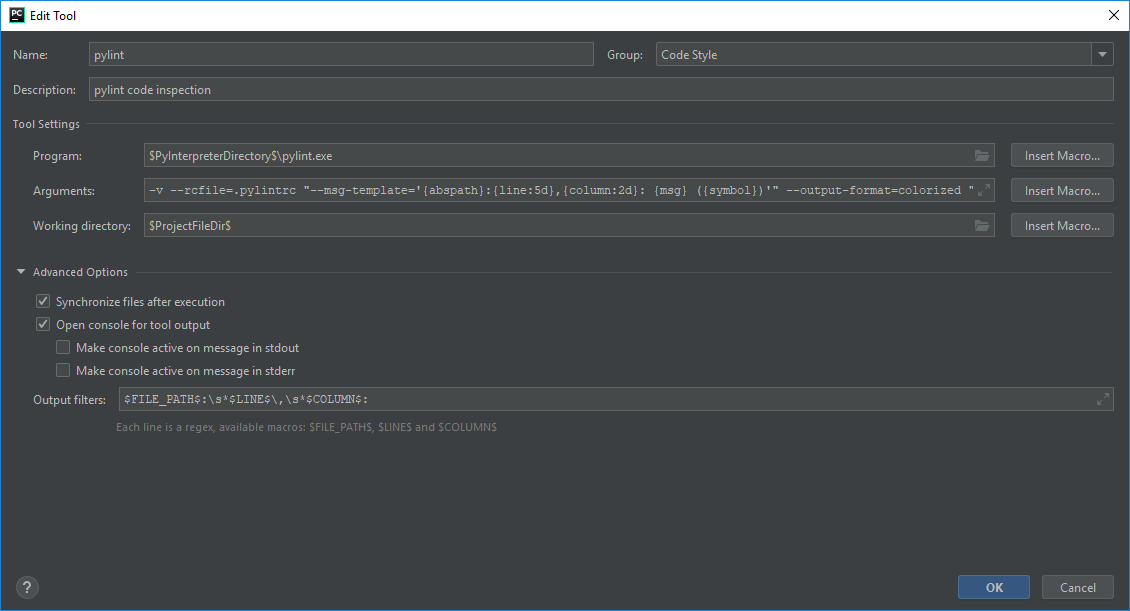
\includegraphics[width=40mm]{ pycharm_pylint_setup.png}

%%%%%%%%%%%%%%%%%%%%%%%%%%%%%%%%%%%%%%%%%%%%%%%%%%%%%%%%%%%%%%%%%%%%%%%%%%%%%%%%%%%%%%%%%%%%%%%%%%%%


\subsection{bandit setup for security testing}

Testing security: bandit
bandit is used to check for common security vulnerabilities

To create a shortcut for the code analysis in pycharm:

\begin{enumerate}
    \item File → Settings
    \item Tools → External Tools
    \item Click the "+" Sign to add a new Tool
    \item Enter the following:
    \begin{itemize}
        \item Name: bandit
        \item Description: Linter for security vulnerabilities
        \item Program: $PyInterpreterDirectory$\bandit
        \item Arguments: -r "$FilePath$"
        \item Working directory: $ProjectFileDir$
        \item Advanced Options
        \begin{itemize}
            \item Syncronize files after execution: True
            \item Open Console for tool Output: True
            \item Output filters: \s*Location:\s*$FILE_PATH$:\s*$LINE$
        \end{itemize}
    \end{itemize}
\end{enumerate}



\begin{yapf setup}
Automatic Code Formatting: yapf
yapf is used for automatic code formatting.

To create a shortcut for the code analysis in pycharm:

\begin{enumerate}
    \item File → Settings
    \item Tools → External Tools
    \item Click the "+" Sign to add a new Tool
    \item Enter the following:
    \begin{itemize}
        \item Name: yapf in-place
        \item Description: Reformat Code in-place
        \item Program: $PyInterpreterDirectory$\yapf.exe
        \item Arguments: --style=yapf.conf -i "$FilePath$"
        \item Working directory: $ProjectFileDir$
        \item Advanced Options
        \begin{itemize}
            \item Syncronize files after execution: True
            \item Open Console for tool Output: True
        \end{itemize}
    \end{itemize}
\end{enumerate}



If you don't want to replace the code in-place remove the -i argument and add another config for that (Lächeln)
